\documentclass{beamer}
\usetheme[hideothersubsections]{HRTheme}
\usepackage{beamerthemeHRTheme}
\usepackage{graphicx}
\usepackage[space]{grffile}
\usepackage{listings}
\lstset{language=SQL,
basicstyle=\ttfamily\footnotesize,
mathescape=true,
keywordstyle=\color{blue},
breaklines=true,
showspaces=false,
showstringspaces=false}
\usepackage[utf8]{inputenc}
\usepackage{color}
\newcommand{\red}[1]{
\textcolor{red}{#1}
}
\newcommand{\ts}{\textbackslash}

\title{Indexing and Query optimization}

\author{ }

\institute{Hogeschool Rotterdam \\ 
Rotterdam, Netherlands}

\date{}

\begin{document}
\maketitle

\SlideSection{Introduction}
\SlideSubSection{Lecture topics}
\begin{slide}{
\item Query optimization.
\item Examples of slow query operations.
\item Hashing.
\item Trees.
}\end{slide}

\SlideSection{Query optimization}
\SlideSubSection{Reasons}
\begin{slide}{
\item Query needs to be fast.
\item Sometimes they are not.
\item You do not want to see your nephew born before retrieving the book you are looking for from Amazon.

\begin{figure}
\centering
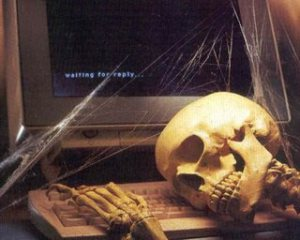
\includegraphics[scale=0.35]{img/skeleton_computer}
\end{figure}
}\end{slide}

\SlideSubSection{Causes}
\begin{slide}{
\item Too much data (Big data analysis).
	\begin{itemize}
	\item Data clustering.
	\item Better hardware. (arrays of disks, caching, ...)
	\end{itemize}
\item Too complex queries (DBMS optimization)
	\begin{itemize}
	\item Refactor query. (Access planner)
	\item Refactor data. (Indexing)
	\end{itemize}
}\end{slide}

\SlideSubSection{Indexes}
\begin{slide}{
\item Query refactoring not always possible.
\item Build additional data to speed up the data retrieval.
}\end{slide}

\SlideSubSection{Indexes}
\begin{slide}{
\item Take your text book and look for the paragraph titled ``Key constraints'' without using the index. How many pages have you looked?
\pause
\item \textbf{Answer:} 29 (from page 3 to 32).
\pause
\item Do the same using the index. How many pages have you looked?
\pause
\textbf{Answer:} 2 (1 in the index, 1 in the text).
}\end{slide}

\SlideSection{Problematic queries}
\begin{frame}[fragile]{Where}
\begin{lstlisting}
SELECT name
FROM ships
WHERE firepower >= 500
\end{lstlisting}
\tiny
\begin{tabular}{|c|c|c|c|c|}
\hline
\multicolumn{5}{|c|}{\textbf{ships}} \\
\hline
name & type & firepower & speed & position \\
\hline
Red 1 & X-Wing & 10 & 300 & (1,3,1) \\
\hline
Red 2 & X-Wing & 10 & 300 & (1,2,1) \\
\hline
Red 3 & X-Wing & 10 & 300 & (0,2.5,1) \\
\hline
Red 4 & X-Wing & 10 & 300 & (2,2.5,1) \\
\hline
Red 5 & X-Wing & 10 & 300 & (2,2.5,0) \\
\hline
Red 6 & X-Wing & 10 & 300 & (2,2.5,0) \\
\hline
Tantine IV & Corellian Corvette & 60 & 300 & (4,2.5,0) \\
\hline
Tyranny & Imperial Star Destroyer & 1500 & 100 & (12,0,0) \\
\hline
Accuser & Imperial Star Destroyer & 1500 & 100& (-12,0,0)\\
\hline
Bombard & Victory Star Destroyer & 500 & 175 & (-6,1,0)\\
\hline
\end{tabular}

\pause
Number of comparisons: 10
\end{frame}

\SlideSection{WHERE}
\begin{slide}{
\item How many comparisons we do at most in a table with R records?
\pause
\item \textbf{R comparisons}
\pause
\item How many comparisons we do at least in a table with R records?
\pause
\item \textbf{R comparisons}
\pause
\item Selection always requires to scan the entire table.
}\end{slide}

\SlideSection{SORTING}
\begin{frame}[fragile]{SORTING}
\begin{itemize}
\item Sorting and grouping requires to sort the column values.
\item The best sorting algorithm requires about $R\log R$ operations, where R is the number of records.
\item Running the query below requires about $10 * \log 10 \simeq 23$ operations.
\end{itemize}

\begin{lstlisting}
SELECT type
FROM ships
WHERE firepower >= 500
ORDER BY firepower DESC
\end{lstlisting}
\end{frame}

\SlideSection{JOIN}
\begin{frame}[fragile]{JOIN}
\begin{itemize}
\item Generate pairs with one element from the first table and the second from the other followed by a selection.
\item Same problem of the selection.
\item Consider the following query applied to ship and the table below.
\end{itemize}

\begin{lstlisting}
SELECT s.name,p.damage
FROM ships s,projectiles p
WHERE s.position = p.position AND
      s.name = p.target
\end{lstlisting}




\tiny
\begin{tabular}{|c|c|c|}
\hline
\multicolumn{3}{|c|}{\textbf{Projectiles}} \\
\hline
target & position & damage \\
\hline
Tantine IV & (0,1,0) & 30 \\
\hline
Tantine IV & (3,1,-2) & 50 \\
\hline
Tantine IV & (4,2.5,0) & 100 \\
\hline
\end{tabular} 
\end{frame}

\SlideSubSection{JOIN performance}
\begin{slide}{
\item How many comparisons does the join make?
\pause
\item Each entity of the first table must be compared.
\item For each entity of the first table there is a comparison with each entity of the second.
\item \textbf{Total comparisons: }$10 \cdot 3 = 30$.
\item How many operations does JOINING two tables, respectively with $N$ and $M$ records, require?
\pause
\item $N \cdot M$.
}\end{slide}



\end{document}

\begin{slide}{
\item ...
}\end{slide}

\begin{frame}[fragile]
\begin{lstlisting}
...
\end{lstlisting}
\end{frame}
